% ============================================================
% Round 09: Image Editing Specific RL
% ============================================================

\subsection{Round 09：图像编辑专属 RL：从“生成好图”到“改对且不乱改”}

\subsubsection{Highlight}

\begin{conceptbox}
\textbf{本章相关论文：}
\begin{itemize}[leftmargin=1.5em]
  \item \textbf{RePlan}：arXiv 2025-12-18，Reasoning-guided Region Planning for Complex Instruction-based Image Editing。核心是 plan-then-execute：先用 VLM planner 把复杂编辑指令分解并定位到区域，再交给 diffusion editor 执行。论文：\url{https://arxiv.org/abs/2512.16864}，项目页：\url{https://replan-iv-edit.github.io/}
  \item \textbf{CogniEdit}：arXiv 2025-12-15，Dense Gradient Flow Optimization for Fine-Grained Image Editing。核心是多模态推理 + Dynamic Token Focus Relocation + Dense GRPO，让连续 denoising steps 有轨迹级监督。论文：\url{https://arxiv.org/abs/2512.13276}
  \item \textbf{ThinkRL-Edit}：arXiv 2026-01-06，v3 2026-02-26，Thinking in Reinforcement Learning for Reasoning-Centric Image Editing。核心是把 reasoning exploration 从 denoising 随机性里拆出来，用 CoT planning / reflection 和 checklist reward 做复杂编辑。论文：\url{https://arxiv.org/abs/2601.03467}
  \item \textbf{UniRef-Image-Edit}：arXiv 2026-02-15，Towards Scalable and Consistent Multi-Reference Image Editing。核心是 SELF 表示和 Multi-Source GRPO，用于多参考图编辑和多图合成。论文：\url{https://arxiv.org/abs/2602.14186}
  \item \textbf{RC-GRPO-Editing}：arXiv 2026-04-10，Region-Constrained Group Relative Policy Optimization for Flow-Based Image Editing。核心是 region-constrained exploration 和 attention concentration reward，减少背景扰动带来的 noisy advantage。论文：\url{https://arxiv.org/abs/2604.09386}
  \item \textbf{HP-Edit}：arXiv 2026-04-21，CVPR 2026，A Human-Preference Post-Training Framework for Image Editing。核心是 RealPref-50K、HP-Scorer、RealPref-Bench，把人类偏好系统化接入图像编辑后训练。论文：\url{https://arxiv.org/abs/2604.19406}
\end{itemize}
\end{conceptbox}

\begin{warnbox}
\textbf{关于代码链接：}\\
RePlan 的 arXiv 页面给出了项目页。其他几篇我目前没有在 arXiv 页面里看到稳定的官方 GitHub 链接；UniRef-Image-Edit 在摘要里说会开源代码、模型、训练数据和 reward 数据，但当前笔记先只记录论文链接。
\end{warnbox}

\subsubsection{为什么图像编辑不能直接照搬文生图 GRPO}

文生图的目标通常是：

\[
\text{prompt } c
\Rightarrow
\text{image } y
\]

它的 reward 可以粗略理解成：

\[
R_\text{t2i}(y,c)
=
\text{文本对齐}
+
\text{视觉质量}
+
\text{美学偏好}
\]

但图像编辑的输入多了原图：

\[
(x,c)
\Rightarrow
y
\]

其中：

\begin{itemize}[leftmargin=1.5em]
  \item $x$ 是原图；
  \item $c$ 是编辑指令；
  \item $y$ 是编辑后的图；
  \item $m$ 是应该被编辑的区域 mask，$1-m$ 是应该保持不变的区域。
\end{itemize}

所以图像编辑的目标不是“生成一张好图”，而是：

\[
\text{改对该改的}
\quad
\text{同时不乱改不该改的}
\]

这可以写成：

\[
R_\text{edit}(y,x,c,m)
=
\lambda_\text{target}R_\text{target}(y,c,m)
+
\lambda_\text{preserve}R_\text{preserve}(y,x,1-m)
+
\lambda_\text{quality}R_\text{quality}(y)
\]

其中：

\[
R_\text{target}
\Rightarrow
\text{编辑区域是否符合指令}
\]

\[
R_\text{preserve}
\Rightarrow
\text{非编辑区域是否保持原图内容}
\]

\[
R_\text{quality}
\Rightarrow
\text{整体是否自然、清晰、没有伪影}
\]

\begin{summarybox}
\textbf{关键转变：}\\
文生图 RL 主要优化：
\[
\text{prompt-image alignment}
\]
图像编辑 RL 还必须同时优化：
\[
\text{instruction following}
\quad
\text{localization}
\quad
\text{source preservation}
\quad
\text{human preference}
\]
这就是为什么会出现图像编辑专属 RL 工作，而不是直接复用 T2I 的 Flow-GRPO。
\end{summarybox}

\subsubsection{编辑任务里的三类失败}

我们先不看论文名字，先看问题本身。图像编辑 RL 主要在修三类失败。

\textbf{第一类：理解失败。}

复杂指令不是简单 prompt，例如：

\[
\text{把左边第二个人的蓝色外套改成红色，但保持背景和其他人不变}
\]

模型需要先知道：

\[
\text{left second person}
\Rightarrow
\text{target instance}
\]

\[
\text{blue coat}
\Rightarrow
\text{target attribute}
\]

\[
\text{red}
\Rightarrow
\text{new attribute}
\]

\[
\text{background and other people}
\Rightarrow
\text{preserve constraints}
\]

如果没有推理和区域规划，模型可能会改错人、改错衣服、或者把背景一起改了。

\textbf{第二类：执行失败。}

就算模型理解了指令，denoising / flow trajectory 里也可能出现：

\[
\text{早期步骤改动范围太大}
\Rightarrow
\text{背景漂移}
\]

\[
\text{中后期步骤局部修正不足}
\Rightarrow
\text{细节没改对}
\]

这时问题不是语义理解，而是 credit assignment：

\[
\text{到底是哪一段 trajectory 导致目标区域没改好？}
\]

\[
\text{到底是哪一段 trajectory 导致非目标区域被污染？}
\]

\textbf{第三类：评价失败。}

图像编辑的 reward 很难写成一个单一分数。假设两个输出：

\[
y_a:
\text{目标改对了，但背景变了}
\]

\[
y_b:
\text{背景保持住了，但目标只改了一半}
\]

哪个更好？这不是普通美学分数能回答的问题。它需要任务相关偏好：

\[
\text{edit success}
\quad
\text{preservation}
\quad
\text{identity consistency}
\quad
\text{naturalness}
\quad
\text{user preference}
\]

\begin{intubox}
\textbf{直觉：}\\
图像编辑 RL 的难点不是“让 reward 变大”这么简单，而是 reward 自身必须知道：哪里应该变，哪里不应该变，什么叫人类真的满意。
\end{intubox}

\subsubsection{主线 A：先推理再编辑}

这一类工作的核心判断是：

\[
\text{复杂编辑失败}
\neq
\text{只是生成模型不够强}
\]

而是：

\[
\text{模型没有先把编辑任务想清楚}
\]

\textbf{RePlan} 的做法是 plan-then-execute：

\[
(x,c)
\xrightarrow{\text{planner}}
z
\xrightarrow{\text{editor}}
y
\]

其中 $z$ 不是图像，而是编辑计划：

\[
z
=
\{
\text{target regions},
\text{sub-instructions},
\text{editing order},
\text{preserve constraints}
\}
\]

RePlan 的重点不是让 diffusion editor 自己猜区域，而是先让 planner 产出 region-aligned plan：

\[
c
\Rightarrow
\text{step-by-step reasoning}
\Rightarrow
\text{region grounding}
\Rightarrow
\text{editor execution}
\]

它还用 GRPO 来强化 planner 的格式可靠性和 reasoning fidelity。也就是说，RL 优化的重点不一定是最终图像模型本身，也可以是：

\[
\pi_\theta(z\mid x,c)
\]

也就是“规划策略”。

\begin{center}
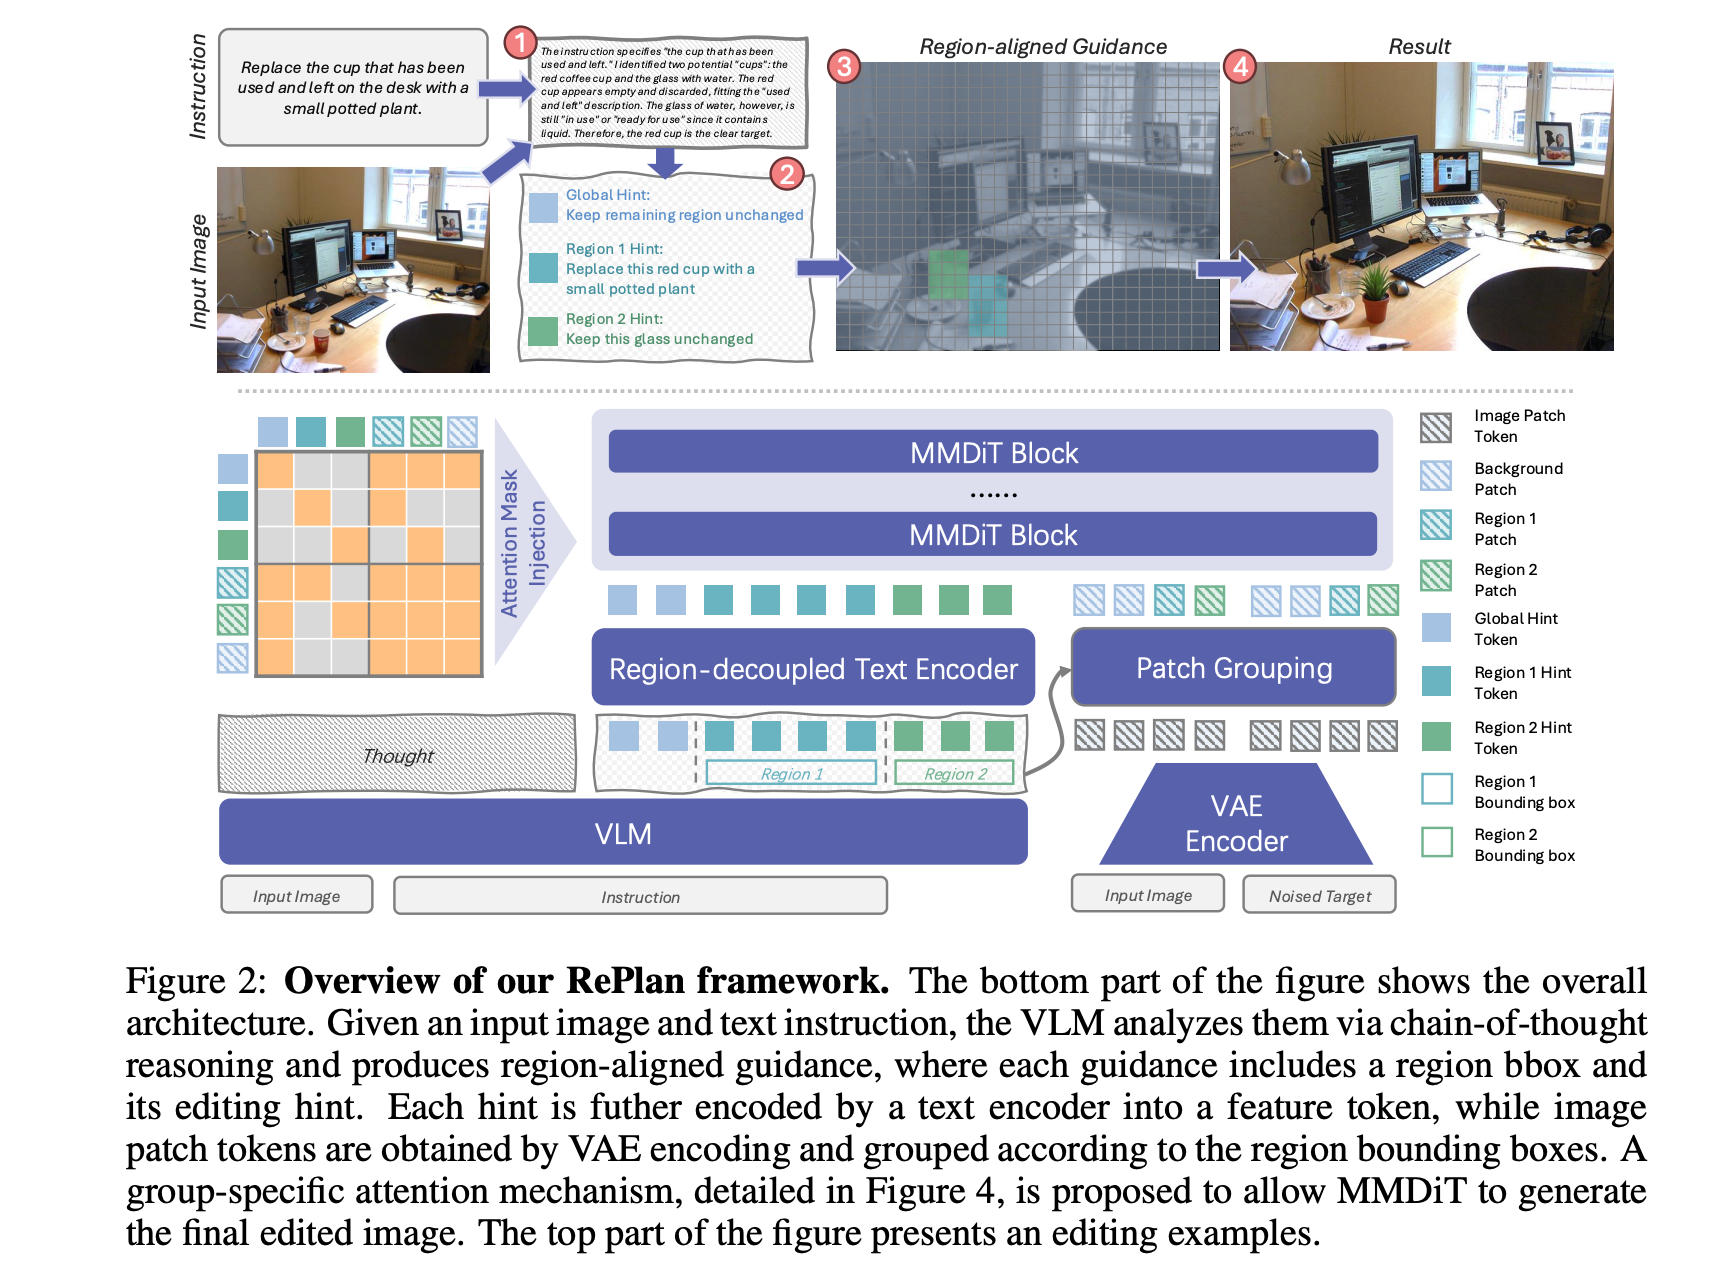
\includegraphics[width=\linewidth]{imgs/replan.png}

{\small\textbf{图：RePlan 架构图。}上半部分是从复杂指令到 region-aligned guidance 再到编辑结果；下半部分是 planner 输出的区域提示如何进入 MMDiT 编辑器。}
\end{center}

这张图可以按 4 步读：

\begin{enumerate}[leftmargin=1.5em]
  \item \textbf{输入：} 左侧给定原图 $x$ 和编辑指令 $c$。例子里不是简单“生成盆栽”，而是要判断哪个 cup 已经用过、哪个 cup 在左边、哪个 glass 需要保持不变。
  \item \textbf{VLM planner：} VLM 先做 thought / chain-of-thought reasoning，把自然语言指令转成结构化的 global hint 和 region hint。
  \item \textbf{Region-aligned guidance：} planner 不只输出文本，还输出每个 region 的 bounding box。于是编辑器知道：
  \[
  \text{Region 1}
  \Rightarrow
  \text{replace red cup with small potted plant}
  \]
  \[
  \text{Region 2}
  \Rightarrow
  \text{keep glass unchanged}
  \]
  \[
  \text{Global}
  \Rightarrow
  \text{keep remaining region unchanged}
  \]
  \item \textbf{MMDiT editor：} 输入图像经过 VAE encoder 变成 image patch tokens；region bbox 把这些 patch 分组；region-decoupled text encoder 把每个 hint 编成对应 token；最后通过 attention mask injection，让不同 region 的 hint 只主要影响自己的 patch group。
\end{enumerate}

因此 RePlan 的关键不是“多加一段提示词”，而是把编辑指令变成：

\[
\text{global hint}
+
\{(\text{bbox}_r,\text{region hint}_r)\}_{r=1}^{R}
\]

也就是：

\[
\text{语言级规划}
\Rightarrow
\text{空间区域绑定}
\Rightarrow
\text{区域级注意力注入}
\Rightarrow
\text{最终编辑}
\]

\begin{intubox}
\textbf{直觉：}\\
普通编辑模型像是“看一句话然后整张图一起改”。RePlan 像是先拿笔在图上圈出每个要处理的区域，再给每个区域单独贴一张小纸条：这里改什么、那里保持什么。这样复杂编辑就不再完全依赖模型自己在隐空间里猜。
\end{intubox}

\textbf{RePlan 细节：Patch Grouping 和 Attention Mask Injection。}

论文里 RePlan 的编辑器基于 MMDiT。普通 MMDiT 会把文本 token、原图 image token、当前 noised latent token 拼成一条序列：

\[
F^\text{text}
=
E_\text{text}(\mathcal{T}),
\qquad
F^\text{img}
=
E_\text{img}(I)
\]

\[
X^{(0)}
=
\left[
F^\text{text}
\;\|\;
F^\text{img}
\;\|\;
\mathbf{z}_t
\right]
\]

其中 $\mathbf{z}_t$ 是当前 diffusion / flow step 的 noisy target latent。

普通 full self-attention 的问题是：

\[
\text{Region 1 的 patch}
\longleftrightarrow
\text{Region 2 的 hint}
\]

也可能发生交互。这样 Region 1 可能被 Region 2 的指令污染，导致 target confusion。

\textbf{第一步：先把 text hint 分组。}

VLM planner 输出：

\[
\{(B_0,h_0),(B_1,h_1),\ldots,(B_K,h_K)\}
\]

其中：

\begin{itemize}[leftmargin=1.5em]
  \item $B_0$ 表示整张图，对应 global hint $h_0$；
  \item $B_k$ 是第 $k$ 个局部编辑区域的 bounding box；
  \item $h_k$ 是第 $k$ 个区域的 editing hint，也可以是 keep unchanged 这种负向提示。
\end{itemize}

这些 hint 不是拼成一句话一起编码，而是分别编码再拼接：

\[
F^\text{text}
=
\left[
E_\text{text}(h_0)
\;\|\;
E_\text{text}(h_1)
\;\|\;
\cdots
\;\|\;
E_\text{text}(h_K)
\right]
\]

于是得到文本 token group：

\[
G^\text{text}_0,\,
G^\text{text}_1,\,
\ldots,\,
G^\text{text}_K
\]

\textbf{第二步：把 image patch 按 bbox 分组。}

原图 $I$ 经过 VAE encoder 后得到二维 feature map，再 reshape 成 patch tokens：

\[
\{f_{i,j}\}_{i=1,\ldots,M;\,j=1,\ldots,N}
\]

每个 bbox $B_k$ 会被映射到这个 patch grid 上：

\[
G^\text{img}_k
=
\left\{
f_{i,j}
\mid
(i,j)\in B_k
\right\},
\qquad
k=1,\ldots,K
\]

背景组就是不属于任何局部 region 的 patch：

\[
G^\text{img}_\text{bg}
=
\{f_{i,j}\}_{i,j}
\setminus
\bigcup_{k=1}^{K}
G^\text{img}_k
\]

\begin{warnbox}
\textbf{注意：}\\
这里的 bbox 不是直接在原始像素上做 attention，而是先映射到 VAE latent / patch grid。也就是说，一个 region 最后对应的是一组 image patch tokens。
\end{warnbox}

\textbf{第三步：在 attention 里注入 mask。}

RePlan 不改 MMDiT 主干参数，也不额外训练 ControlNet 之类的模块，而是在每一层 attention 里加入一个二值 mask：

\[
M
\in
\{0,1\}^{|X|\times |X|}
\]

如果：

\[
M_{u,v}=1
\]

表示 token $u$ 可以 attend to token $v$。如果：

\[
M_{u,v}=0
\]

表示这条 attention 边被屏蔽。

可以把 masked attention 写成：

\[
\text{Attn}_M(u)
=
\sum_v
\text{softmax}_v
\left(
\frac{q_u k_v^\top}{\sqrt{d}}
+
b_{u,v}
\right)
v_v
\]

其中：

\[
b_{u,v}
=
\begin{cases}
0, & M_{u,v}=1 \\
-\infty, & M_{u,v}=0
\end{cases}
\]

这样 mask 不是在输出图像上后处理，而是直接改变 Transformer 内部的信息流。

\textbf{第四步：mask 遵守 5 条规则。}

\begin{enumerate}[leftmargin=1.5em]
  \item \textbf{组内互通：} 同一个 group 内部的 token 可以互相 attend。这样每个文本组、每个图像区域、每个 latent 区域内部不会被切碎。
  \item \textbf{Hint isolation：} 不同 text hint group 之间不互相 attend：
  \[
  G^\text{text}_a
  \not\leftrightarrow
  G^\text{text}_b,
  \qquad
  a\neq b
  \]
  这样 Region 1 的提示不会污染 Region 2 的提示。
  \item \textbf{Image--latent full interaction：} image tokens 和 latent tokens 保持全局连接。论文强调不能把图像不同区域之间完全切断，否则区域边缘会出现明显割裂，整体一致性会变差。
  \item \textbf{Region constraint：} 属于第 $k$ 个区域的 image patch 只看自己的 hint 和 global hint：
  \[
  u\in G^\text{img}_k
  \Rightarrow
  u
  \text{ can attend to }
  G^\text{text}_k
  \cup
  G^\text{text}_0
  \]
  这样局部编辑既受自己的区域指令控制，也不会丢掉全局风格 / 背景约束。
  \item \textbf{Background constraint：} 背景 patch 只看 global hint：
  \[
  u\in G^\text{img}_\text{bg}
  \Rightarrow
  u
  \text{ can attend to }
  G^\text{text}_0
  \]
  这样背景不会被局部编辑提示污染。
\end{enumerate}

论文附录还补了两个细节：

\begin{itemize}[leftmargin=1.5em]
  \item \textbf{bbox 重叠：} 如果两个 bbox 重叠，重叠 patch 可以同时 attend 到对应的多个 hint。因为 image patch 之间仍保留 full self-attention，模型可以自己协调这些 sub-edits。
  \item \textbf{bbox 扰动鲁棒性：} 只要 bbox 还大致对应正确目标，像素级误差影响不大；论文做了 bbox corner 随机 scale / shift 扰动实验，直到较大扰动前整体分数仍较稳定。
\end{itemize}

\begin{summarybox}
\textbf{RePlan attention injection 的本质：}\\
它不是简单地“把区域提示拼进 prompt”，而是把文本 hint 和图像 patch 都分组，然后用 attention mask 规定信息流：
\[
\text{每个编辑区域}
\longleftrightarrow
\text{自己的 hint}
\quad
\text{背景}
\longleftrightarrow
\text{global hint}
\]
同时保留 image--latent 的全局交互，避免区域边界割裂。
\end{summarybox}

\textbf{ThinkRL-Edit} 更进一步，把 reasoning exploration 从 denoising 随机性里拿出来。普通图像 RL 的探索主要来自：

\[
\epsilon_t
\sim
\mathcal{N}(0,I)
\]

也就是采样噪声。但复杂编辑里，更关键的探索其实是：

\[
\text{我该如何理解这条指令？}
\]

\[
\text{我该先改什么、后改什么？}
\]

\[
\text{这个编辑计划是否和原图语义一致？}
\]

所以 ThinkRL-Edit 把策略拆成：

\[
\pi_\theta(z,y\mid x,c)
=
\pi_\theta(z\mid x,c)
\pi_\theta(y\mid x,c,z)
\]

其中 $z$ 是 reasoning chain / plan / reflection。

这样 GRPO 优化的不只是图像输出，还包括：

\[
\text{reasoning chain 的质量}
\Rightarrow
\text{最终编辑质量}
\]

\begin{center}
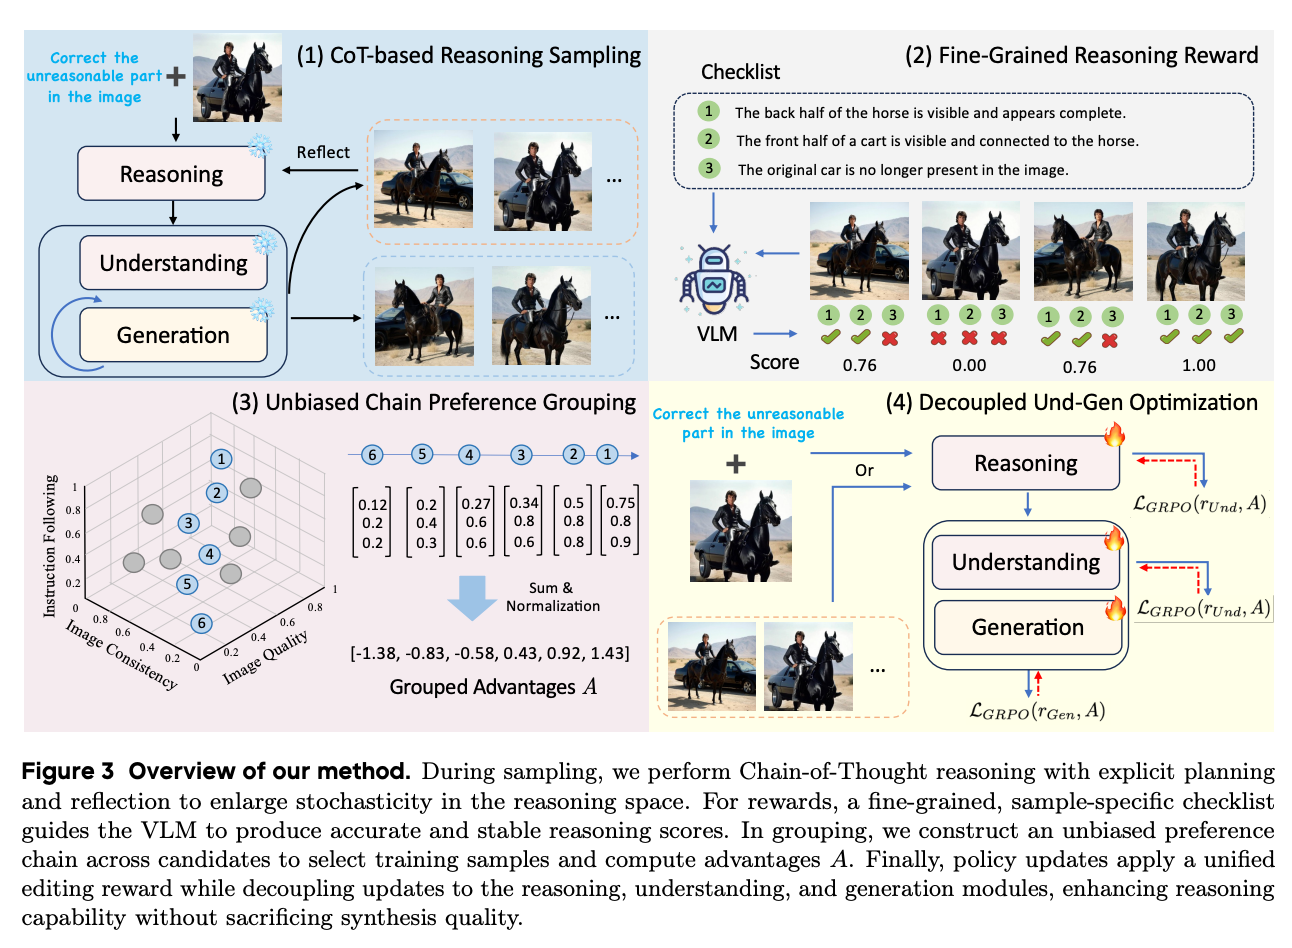
\includegraphics[width=\linewidth]{imgs/thinkRL.png}

{\small\textbf{图：ThinkRL-Edit 架构图。}它把 reasoning sampling、checklist reward、unbiased chain preference grouping、decoupled Und-Gen optimization 放在同一个 RL 闭环里。}
\end{center}

这张图可以按 4 个模块读。

\textbf{模块 1：CoT-based Reasoning Sampling。}

普通 Flow-GRPO 的探索主要发生在 denoising / flow trajectory：

\[
x_t
\rightarrow
x_{t-1}
\rightarrow
\cdots
\rightarrow
x_0
\]

也就是改变采样噪声。但 ThinkRL-Edit 认为 reasoning-centric editing 的关键随机性应该发生在语义空间：

\[
\text{reasoning path}
\rightarrow
\text{understanding}
\rightarrow
\text{generation}
\]

论文算法里，初始 policy 被拆成：

\[
\pi_\theta
=
\left(
\pi_\theta^\text{Und},
\pi_\theta^\text{Gen}
\right)
\]

给定输入图像 $\mathbf{p}$ 和编辑指令 $\mathbf{c}$，先用旧的 understanding policy 生成 reasoning-enhanced prompt：

\[
\mathbf{c}'
\sim
\pi_{\theta_\text{old}}^\text{Und}
(\cdot\mid \mathbf{p},\mathbf{c})
\]

然后用 $\mathbf{c}'$ 生成第一批 $G$ 个编辑结果：

\[
\{\mathbf{o}_i\}_{i=1}^{G}
\sim
\pi_{\theta_\text{old}}
(\cdot\mid \mathbf{p},\mathbf{c}')
\]

接着模型对这些结果做一次 reflection，得到反思后的 prompt：

\[
\mathbf{c}''_i
\sim
\pi_{\theta_\text{old}}^\text{Und}
(\cdot\mid \mathbf{o}_i,\mathbf{p},\mathbf{c}')
\]

再用 $\mathbf{c}''$ 生成第二批 reflected samples：

\[
\{\mathbf{o}_i\}_{i=G+1}^{2G}
\sim
\pi_{\theta_\text{old}}
(\cdot\mid \mathbf{p},\mathbf{c}'')
\]

所以它不是只采样不同图像，而是采样不同“思考路径”和“反思路径”。

\begin{intubox}
\textbf{直觉：}\\
Flow-GRPO 是在“怎么画”上探索；ThinkRL-Edit 还要在“怎么理解这条编辑指令”上探索。复杂编辑里，理解错了，后面的生成轨迹再怎么优化也只是把错误画得更漂亮。
\end{intubox}

\textbf{模块 2：Fine-Grained Reasoning Reward。}

普通 VLM reward 常见做法是让 VLM 给一个区间分：

\[
\text{score}
\in
\{1,2,3,4,5\}
\]

ThinkRL-Edit 认为这种 interval score 在复杂推理编辑里不稳定，于是改成 sample-specific checklist。比如图里的指令是修正图像中不合理部分，checklist 会拆成：

\[
\begin{aligned}
q_1 &: \text{马的后半身是否完整可见？}\\
q_2 &: \text{车的前半部分是否可见并且连接到马？}\\
q_3 &: \text{原来的汽车是否已经不在图中？}
\end{aligned}
\]

VLM 不再给模糊分数，而是对每个问题回答 yes / no。对第 $i$ 个样本：

\[
R_\text{check}(\mathbf{o}_i)
=
\frac{1}{M}
\sum_{m=1}^{M}
\mathbb{I}
\left[
\text{VLM says yes to } q_m
\right]
\]

图中每张候选图下面的 0.76、0.00、1.00，就是 checklist 通过率式的分数。

\textbf{模块 3：Unbiased Chain Preference Grouping。}

图像编辑的 reward 不是一维的。论文同时看：

\[
\text{Instruction Following}
\quad
\text{Image Consistency}
\quad
\text{Image Quality}
\]

如果直接加权：

\[
R_i
=
\sum_{k=1}^{K}
w_k r_i^k
\]

权重 $w_k$ 会引入偏置。比如 consistency 权重大，模型可能什么都不改；instruction 权重大，模型可能过度编辑。

ThinkRL-Edit 的做法是保留多维 reward：

\[
\mathbf{r}_i
=
\left(
r_i^1,
r_i^2,
\ldots,
r_i^K
\right)
\]

然后找一条在多个维度上排序一致的 preference chain：

\[
\mathbf{r}_{i_1}
\preceq
\mathbf{r}_{i_2}
\preceq
\cdots
\preceq
\mathbf{r}_{i_N}
\]

也就是：被放进同一条链的样本，不能是“这个样本 instruction 高但 quality 低，另一个 quality 高但 consistency 低”这种互相打架的关系。链上的样本才参与 advantage 计算。

论文算法里，对链上第 $i$ 个样本：

\[
A_i
=
\frac{
\sum_{k=1}^{K}r_i^k
-
K\mu
}{
K\sigma
}
\]

其中 $\mu,\sigma$ 是当前 preference chain 上的均值和标准差统计。

\begin{warnbox}
\textbf{为什么叫 unbiased：}\\
它不是说完全没有偏差，而是相对“手写权重加权求和”更少引入人为目标偏置。只有在多个 reward 维度上形成一致偏好顺序的样本，才被用来更新策略。
\end{warnbox}

\textbf{模块 4：Decoupled Und-Gen Optimization。}

普通 Flow-GRPO 只更新 generation trajectory：

\[
r_{\text{Gen},t}^{i}
=
\frac{
p_\theta(x_{t-1}^i\mid x_t^i,c)
}{
p_{\theta_\text{old}}(x_{t-1}^i\mid x_t^i,c)
}
\]

ThinkRL-Edit 还要更新 understanding / reasoning 侧。对第 $i$ 条 reasoning / understanding token 序列 $y^i$，它计算：

\[
r_\text{Und}^{i}
=
\frac{
p_\theta^\text{Und}(y^i\mid x)
}{
p_{\theta_\text{old}}^\text{Und}(y^i\mid x)
}
\]

展开就是整段 token logprob 的差：

\[
r_\text{Und}^{i}
=
\exp
\left(
\sum_t
\log p_\theta^\text{Und}
(y_t^i\mid x,y_{<t}^{i})
-
\sum_t
\log p_{\theta_\text{old}}^\text{Und}
(y_t^i\mid x,y_{<t}^{i})
\right)
\]

于是同一个 grouped advantage $A_i$ 会用于两类更新：

\[
\mathcal{J}_\text{Und}
=
\mathbb{E}
\left[
f(r_\text{Und},A)
\right]
\]

\[
\mathcal{J}_\text{Gen}
=
\mathbb{E}
\left[
f(r_\text{Gen},A)
\right]
\]

图里右下角的火焰符号就在表示：reasoning / understanding / generation 都会被 GRPO loss 更新，但它们用的 ratio 不同。

\begin{summarybox}
\textbf{ThinkRL-Edit 的核心：}\\
它把图像编辑策略从单一的“生成策略”扩展成：
\[
\text{理解 / 推理策略}
\quad
+
\quad
\text{图像生成策略}
\]
再用 checklist reward 和 unbiased preference chain 给这两部分共同分配 advantage。这样 RL 优化的不只是“生成结果像不像”，而是“推理路径是否帮助最终编辑成功”。
\end{summarybox}

\begin{summarybox}
\textbf{这条主线的核心：}\\
RePlan 和 ThinkRL-Edit 都在说：复杂图像编辑不能只靠 denoising 随机性探索。更重要的是先把编辑任务变成显式 plan，再用 RL 奖励好的 plan。
\end{summarybox}

\subsubsection{主线 B：细粒度编辑需要 dense trajectory supervision}

如果指令是：

\[
\text{把杯子左侧的小蓝色 logo 改成黄色}
\]

模型不仅要理解目标，还要在采样轨迹里持续关注这个细节。

普通 GRPO 常见做法是：采样 $G$ 个结果，计算最终 reward：

\[
R_1,\ldots,R_G
\]

再得到组内 advantage：

\[
A_i
=
\frac{
R_i-\text{mean}(R_1,\ldots,R_G)
}{
\text{std}(R_1,\ldots,R_G)+\epsilon
}
\]

问题是：同一个 $A_i$ 被分配给整条生成轨迹。

\[
A_i
\Rightarrow
\{t_1,t_2,\ldots,t_K\}
\]

但细粒度编辑里，不同时间步做的事情不一样：

\[
\text{early steps}
\Rightarrow
\text{布局和大结构}
\]

\[
\text{middle steps}
\Rightarrow
\text{目标属性和局部形状}
\]

\[
\text{late steps}
\Rightarrow
\text{纹理、边缘、细节}
\]

\textbf{CogniEdit} 针对的就是这个问题。它认为只在单个 sampling step 上优化，反馈太稀疏，不能形成 trajectory-level control。

可以把它的思想抽象成：

\[
\text{instruction}
\Rightarrow
\text{actionable directives}
\Rightarrow
\text{token focus}
\Rightarrow
\text{dense GRPO over consecutive steps}
\]

也就是：

\[
A_{i,k:k+h}
\Rightarrow
\{t_k,t_{k+1},\ldots,t_{k+h}\}
\]

而不是只把一个最终分数硬塞给所有步骤。

动态 token focus 的作用是：当指令里出现颜色、数量、位置等细节时，让模型在相关 token / region 上投入更多优化信号：

\[
\text{blue}
\quad
\text{left}
\quad
\text{two}
\quad
\text{small logo}
\]

这些词不是普通 prompt token，而是编辑成功与否的关键属性。

\textbf{CogniEdit 细节一：先把复杂指令变成可执行指令。}

CogniEdit 认为细粒度编辑失败的第一层原因是 understanding gap：

\[
\text{用户原始指令}
\not\Rightarrow
\text{模型能直接执行的视觉约束}
\]

比如：

\[
\text{Change the car to a sports car}
\]

里面隐含了：

\[
\text{low profile}
\quad
\text{aerodynamic shape}
\quad
\text{sporty visual features}
\]

普通编辑模型可能只知道“换成车”，但不知道 sports car 应该长什么样。

所以 CogniEdit 先用 MLLM 做 instruction enhancement。它把复杂指令拆成：

\[
\text{semantic decomposition}
\quad
\text{knowledge injection}
\quad
\text{spatial grounding}
\]

论文补充材料里给了结构化输出形式，可以理解成：

\[
\text{\texttt{<info>}}
\Rightarrow
\text{图像描述}
\]

\[
\text{\texttt{<think>}}
\Rightarrow
\text{推理过程}
\]

\[
\text{\texttt{<answer>}}
\Rightarrow
\text{增强后的编辑指令}
\]

\[
\text{\texttt{<object>}}
\Rightarrow
\text{目标对象 / 区域说明}
\]

也就是：

\[
(x,c)
\xrightarrow{\text{MLLM}}
c^\star
\]

其中 $c^\star$ 是更明确、更细粒度、更有视觉知识的编辑指令。

\begin{intubox}
\textbf{直觉：}\\
RePlan 偏向“把区域规划出来”，ThinkRL-Edit 偏向“让模型先思考再反思”，CogniEdit 这里偏向“把原始指令翻译成模型更容易执行的细粒度视觉指令”。
\end{intubox}

\textbf{CogniEdit 细节二：GRPO for Image Editing 不是直接照搬 Flow-GRPO。}

CogniEdit 指出，编辑模型常用 deterministic ODE 来保证一致性：

\[
x_{t+\Delta t}
=
x_t
+
s_\theta(x_t,t)\Delta t
\]

但如果完全确定性，同一个输入采样 $G$ 次会得到几乎一样的结果：

\[
x_0^1
\approx
x_0^2
\approx
\cdots
\approx
x_0^G
\]

这会让 GRPO 的组内比较失去意义。

所以它沿用 Flow-GRPO 思路，引入受控随机性：

\[
x_{t+\Delta t}
=
x_t
+
s_\theta(x_t,t)\Delta t
+
\sqrt{\Delta t}\sigma_t\epsilon
\]

其中：

\[
\epsilon
\sim
\mathcal{N}(0,I)
\]

而：

\[
s_\theta(x_t,t)
=
v_\theta(x_t,t)
+
\frac{\sigma_t^2}{2}
\left[
x_t
+
(1-t)v_\theta(x_t,t)
\right]
\]

这一步的作用是：

\[
\text{deterministic edit}
\Rightarrow
\text{可产生组内差异的 stochastic edit}
\]

但 CogniEdit 又发现：图像编辑同一个输入下的组内差异仍然有限，如果只在同一个样本内部归一化 advantage，方差会很大。

所以它用 batch-level advantage。设一个 batch 有 $B$ 个编辑任务，每个任务采样 $G$ 个结果：

\[
\{x_0^{b,i}\},
\qquad
b=1,\ldots,B,
\quad
i=1,\ldots,G
\]

batch reward 均值是：

\[
\mu_\text{batch}
=
\frac{1}{BG}
\sum_{b=1}^{B}
\sum_{i=1}^{G}
R(x_0^{b,i},c_b)
\]

batch 标准差是：

\[
\sigma_\text{batch}
=
\text{std}
\left(
\{R(x_0^{b,i},c_b)\}_{b,i}
\right)
\]

第 $b$ 个编辑任务的 advantage 写成：

\[
\hat{A}^{b}
=
\frac{1}{G}
\sum_{i=1}^{G}
\frac{
R(x_0^{b,i},c_b)
-
\mu_\text{batch}
}{
\sigma_\text{batch}
}
\]

这和普通 GRPO 的区别是：

\[
\text{普通 GRPO：同 prompt 组内归一化}
\]

\[
\text{CogniEdit：跨 batch 的编辑结果一起做统计}
\]

这样对编辑任务更稳，因为编辑任务的组内 diversity 天然比文生图小。

\textbf{CogniEdit 细节三：Dynamic Token Focus Relocation。}

CogniEdit 观察到，模型容易一直关注：

\[
\text{change}
\quad
\text{add}
\quad
\text{replace}
\]

这些 generic action words，却忽略真正决定编辑是否成功的属性词：

\[
\text{purple}
\quad
\text{five}
\quad
\text{on the left}
\quad
\text{in the background}
\]

所以它不是固定强调某些 token，而是让不同层动态选择要关注的 token。

设第 $i$ 层的 instruction token 表示为：

\[
h_i^l
\in
\mathbb{R}^{l\times d}
\]

其中 $l$ 是 token 数，$d$ 是 hidden dimension。CogniEdit 加一个轻量 predictor：

\[
\text{pos}
=
p_\eta(h_i^l),
\qquad
\text{pos}\in[0,l-\xi]
\]

这里 $\xi$ 是要强调的连续 token 数。

然后给每一层一个可学习 soft token：

\[
s_i^{1:\xi}
=
E(i)
\in
\mathbb{R}^{\xi\times d}
\]

把原来位置上的 token embedding 替换为 soft token：

\[
h_i^{\text{pos}:\text{pos}+\xi}
\leftarrow
s_i^{1:\xi}
\]

再用这些 soft token 去影响 attention：

\[
a_i^{\text{pos}:\text{pos}+\xi}
=
s_i^{1:\xi}
\cdot
A^l
\]

这里沿用论文里的记号，$A^l$ 表示对应层的 attention map。不要把这个 $l$ 和上面的 token 长度死扣，核心是：soft token 被放到某个预测位置后，会成为这一层的 attention anchor。

这套机制的直觉是：

\[
\text{early layers}
\Rightarrow
\text{high-level semantics}
\]

\[
\text{deep layers}
\Rightarrow
\text{fine-grained attributes}
\]

所以不同层应该关注不同指令成分。它不是手动指定“蓝色重要”，而是让 predictor 和 soft tokens 在训练中学会：

\[
\text{哪个层该看哪个 token}
\]

\begin{warnbox}
\textbf{注意：}\\
Dynamic Token Focus Relocation 不是简单 prompt reweighting。它是在模型内部每一层动态重定位 token focus，并用 learnable soft tokens 当 attention anchor。
\end{warnbox}

\textbf{CogniEdit 细节四：Dense GRPO 是连续 $k$ 步的 ratio，而不是单步 ratio。}

标准 Flow-GRPO 的 objective 会在每个 timestep 上使用单步 ratio：

\[
r_i^t(\theta)
=
\frac{
p_\theta(x_{t-1}^i\mid x_t^i,c)
}{
p_{\theta_\text{old}}(x_{t-1}^i\mid x_t^i,c)
}
\]

CogniEdit 认为这样仍然太碎，而且不能让梯度沿连续采样轨迹传播。

它随机选择一个能连续去噪 $k$ 步的起始 timestep。按照我们这里的写法：

\[
r
\in
\{k,\ldots,T\}
\]

这样才能从 $x_r$ 合法地走到 $x_{r-k}$。如果另一篇论文把时间索引反过来，也可能写成 $r\in[0,T-k]$，本质都是“选一段长度为 $k$ 的连续 denoising window”。

然后连续跑 $k$ 个 denoising steps：

\[
x_r
\rightarrow
x_{r-1}
\rightarrow
\cdots
\rightarrow
x_{r-k}
\]

单步更新写成：

\[
x_{t-1}
=
x_t
-
\frac{1}{T}
s_\theta(\text{sg}(x_t),t)
+
\frac{\sigma_t}{\sqrt{T}}\epsilon
\]

这里：

\[
\text{sg}(\cdot)
\]

是 stop-gradient。它的作用是稳定梯度路径，避免后续“补完图像”的过程把梯度乱传回不该更新的地方。

对这连续 $k$ 步，CogniEdit 不再只算单步 ratio，而是算整段 log-ratio。为了避免倒序求和的歧义，可以把它写成：

\[
\psi_b^{r:r-k}(\theta)
=
\sum_{j=0}^{k-1}
\log
\frac{
p_\theta(x_{r-j-1}^{b}\mid x_{r-j}^{b},c_b)
}{
p_{\theta_\text{old}}(x_{r-j-1}^{b}\mid x_{r-j}^{b},c_b)
}
\]

也就是把连续 $k$ 步的 ratio 先相乘：

\[
r_b^{r:r-k}(\theta)
=
\prod_{j=0}^{k-1}
\frac{
p_\theta(x_{r-j-1}^{b}\mid x_{r-j}^{b},c_b)
}{
p_{\theta_\text{old}}(x_{r-j-1}^{b}\mid x_{r-j}^{b},c_b)
}
\]

再取 log 变成求和，数值更稳定。

再把它转成 trajectory-level clipped ratio：

\[
\tilde{r}_b^{r:r-k}(\theta)
=
\exp
\left(
\text{clip}
\left(
\psi_b^{r:r-k}(\theta),
-\log(1+\epsilon),
\log(1+\epsilon)
\right)
\right)
\]

最终 Dense GRPO objective 是：

\[
\begin{aligned}
\mathcal{J}_\text{Dense}(\theta)
&=
\mathbb{E}
\Bigg[
\frac{1}{B}
\sum_{b=1}^{B}
\min
\Big(
\tilde{r}_b^{r:r-k}\hat{A}^{b},
\\
&\quad
\text{clip}
\left(
\tilde{r}_b^{r:r-k},
1-\epsilon,
1+\epsilon
\right)
\hat{A}^{b}
\Big)
-
\hat{\beta}
D_\text{KL}
(\pi_\theta\|\pi_\text{ref})
\Bigg]
\end{aligned}
\]

这里的 $\hat{A}^{b}$ 不是在 $x_{r-k}$ 这个中间态上直接算的，而是继续 denoise 到完整结果 $x_0$ 后，用最终 reward 来算。论文里的训练流程是：

\[
x_r
\xrightarrow{k\text{ steps}}
x_{r-k}
\xrightarrow{\text{stop-gradient complete}}
x_0
\xrightarrow{R}
\hat{A}^{b}
\]

\textbf{CogniEdit 细节五：reward 不是 CLIP，而是 MLLM 多维评价。}

CogniEdit 的最终 reward 来自 Qwen2.5-VL-7B-Instruct 这类 MLLM evaluator。输入是：

\[
(\text{edited image},\text{original image},\text{editing instruction})
\]

它先做 word-level analysis，检查 instruction 里的 subject、object、color、number、lighting、style、activity 等元素有没有被正确体现；然后给多个维度打分：

\[
S_\text{alignment}
\quad
S_\text{coherence}
\quad
S_\text{style}
\quad
S_\text{consistency}
\]

其中：

\[
S_\text{alignment}
\Rightarrow
\text{是否符合指令}
\]

\[
S_\text{coherence}
\Rightarrow
\text{是否逻辑一致、无明显伪影、无数量/颜色错误}
\]

\[
S_\text{consistency}
\Rightarrow
\text{是否保持原图未编辑区域}
\]

论文没有把 style score 放进最终 reward，因为 style 更像审美质量，可能和编辑正确性无关。最终 reward 可以写成：

\[
R
=
S_\text{alignment}
+
S_\text{coherence}
+
S_\text{consistency}
\]

所以 CogniEdit 的 reward 对应的是：

\[
\text{改对}
\quad
\text{改得合理}
\quad
\text{不乱改}
\]

而不是单纯：

\[
\text{图像好看}
\]

\begin{summarybox}
\textbf{CogniEdit 的核心不是一句“dense reward”：}\\
它实际做了三件事：
\[
\text{MLLM 指令增强}
\Rightarrow
\text{layer-wise token focus}
\Rightarrow
\text{连续 } k \text{ 步 Dense GRPO}
\]
其中 Dense GRPO 的关键是整段 trajectory ratio $\tilde{r}_b^{r:r-k}$，而不是把最终 reward 简单平均分给每一步。
\end{summarybox}

\begin{intubox}
\textbf{直觉：}\\
CogniEdit 关心的是“细节到底在哪个步骤被改坏或改好”。它不是只问最终图像好不好，而是让 reward 信号沿着连续 denoising steps 更密地传回去。
\end{intubox}

\subsubsection{主线 C：区域约束的 GRPO}

图像编辑和文生图最大的区别在这里：

\[
\text{编辑区域应该变化}
\]

\[
\text{非编辑区域应该不变}
\]

如果我们仍然做全局探索：

\[
x_T
=
x_T^\text{base}
+
\sigma\epsilon
\]

那么 $\epsilon$ 会影响整张图。结果是：

\[
\text{目标区域变化}
+
\text{背景随机漂移}
\]

这会污染 reward。

设总 reward 是：

\[
R
=
R_\text{target}
+
R_\text{background}
\]

组内方差是：

\[
\text{Var}(R)
=
\text{Var}(R_\text{target})
+
\text{Var}(R_\text{background})
+
2\text{Cov}(R_\text{target},R_\text{background})
\]

我们真正想利用的是：

\[
\text{Var}(R_\text{target})
\]

因为它告诉我们目标区域哪个样本更好。

但全局探索会让：

\[
\text{Var}(R_\text{background})
\]

变大。这样 advantage 就变噪：

\[
A_i
=
\frac{R_i-\bar{R}}{\text{std}(R)+\epsilon}
\]

里面的 $R_i$ 不再只反映编辑好坏，还混进了背景漂移。

\textbf{RC-GRPO-Editing} 的思想是：探索也应该局部化。

可以抽象成：

\[
\epsilon
=
m\odot\epsilon_\text{edit}
+
(1-m)\odot\epsilon_\text{bg}
\]

并让：

\[
\|\epsilon_\text{bg}\|
\ll
\|\epsilon_\text{edit}\|
\]

这样随机性主要发生在编辑区域，而不是整张图。

它还引入 attention concentration reward，让 cross-attention 更集中到目标区域。可以写成：

\[
R_\text{attn}
=
\frac{
\sum_{p\in m}A(p)
}{
\sum_{p}A(p)+\epsilon
}
\]

其中 $A(p)$ 表示目标编辑 token 对空间位置 $p$ 的 attention mass。

如果模型注意力扩散到背景：

\[
R_\text{attn}
\downarrow
\]

如果模型注意力集中在编辑区域：

\[
R_\text{attn}
\uparrow
\]

\begin{summarybox}
\textbf{RC-GRPO-Editing 的核心问题：}\\
普通 GRPO 的组内比较假设“组内差异主要来自任务相关探索”。但图像编辑里，全局探索会制造大量背景差异。RC-GRPO-Editing 的目标是把探索和 credit 都限制在该编辑的区域里。
\end{summarybox}

\subsubsection{主线 D：人类偏好怎么进入图像编辑}

前面几条主线主要在修算法：

\[
\text{planning}
\quad
\text{dense credit}
\quad
\text{region-constrained exploration}
\]

但还有一个更基础的问题：

\[
\text{reward 到底从哪里来？}
\]

图像编辑的偏好不是一个简单标签。人类看编辑结果时，通常同时看：

\[
\text{是否按指令改了}
\]

\[
\text{原图身份 / 背景 / 风格是否保留}
\]

\[
\text{结果是否自然}
\]

\[
\text{有没有过度编辑}
\]

\textbf{HP-Edit} 做的是把人类偏好数据、自动 scorer、benchmark 连接起来：

\[
\text{human preference data}
\Rightarrow
\text{HP-Scorer}
\Rightarrow
\text{reward for post-training}
\Rightarrow
\text{RealPref-Bench evaluation}
\]

偏好数据可以抽象成：

\[
\mathcal{D}_\text{pref}
=
\{
(x,c,y^+,y^-)
\}
\]

其中 $y^+$ 是人更喜欢的编辑结果，$y^-$ 是相对更差的结果。

训练 scorer：

\[
s_\phi(x,c,y)
\]

使得：

\[
s_\phi(x,c,y^+)
>
s_\phi(x,c,y^-)
\]

然后后训练时直接把 scorer 当 reward：

\[
R(y,x,c)
=
s_\phi(x,c,y)
\]

这样图像编辑 RL 就不再依赖零散的 CLIP / aesthetic / VLM 打分，而是有一个更贴近真实编辑偏好的 reward。

\begin{warnbox}
\textbf{注意：}\\
HP-Edit 解决的不是“GRPO 公式怎么改”，而是“图像编辑的 reward model 和 benchmark 怎么建立”。没有可靠 reward，再精巧的 RL 算法也只是在优化错误目标。
\end{warnbox}

\subsubsection{主线 E：多参考图编辑}

单图编辑是：

\[
(x,c)
\Rightarrow
y
\]

多参考图编辑是：

\[
(x^{(1)},x^{(2)},\ldots,x^{(n)},c)
\Rightarrow
y
\]

比如：

\[
\text{用图 1 的人物，穿图 2 的衣服，站在图 3 的场景里}
\]

这里的问题是 reference 之间可能冲突：

\[
x^{(1)}
\Rightarrow
\text{人物身份}
\]

\[
x^{(2)}
\Rightarrow
\text{服装风格}
\]

\[
x^{(3)}
\Rightarrow
\text{背景光照}
\]

如果这些约束互相不一致，模型必须学会取舍和融合。

\textbf{UniRef-Image-Edit} 的关键是 SELF：

\[
\text{Sequence-Extended Latent Fusion}
\]

把多个 reference 动态序列化成一个统一 latent sequence：

\[
\{x^{(1)},\ldots,x^{(n)}\}
\Rightarrow
z_\text{SELF}
\]

并在固定 pixel budget 下训练模型处理不同数量、不同分辨率、不同作用的参考图。

RL 阶段则使用 Multi-Source GRPO：

\[
\text{MSGRPO}
\]

它的目标不是只让输出符合一个 prompt，而是协调多个 source constraints：

\[
R
=
\sum_{j=1}^{n}
\lambda_j R_j(y,x^{(j)},c)
\]

其中 $R_j$ 可以对应身份、物体、姿态、风格、背景等不同参考源。

\begin{intubox}
\textbf{直觉：}\\
多参考图编辑的本质是“多条件约束优化”。MSGRPO 不是单纯奖励最终图好不好，而是让模型学会在多个 reference 之间做一致性协调。
\end{intubox}

\subsubsection{这一章的统一框架}

现在把这几篇论文放到同一个框架里：

\begin{center}
{\small
\begin{tabular}{p{3.2cm}p{4.2cm}p{5.4cm}}
\hline
\textbf{论文} & \textbf{主要解决的问题} & \textbf{对应的抽象模块} \\
\hline
RePlan
&
复杂指令需要区域规划
&
$\pi_\theta(z\mid x,c)$：先生成 region-aligned plan
\\
ThinkRL-Edit
&
复杂编辑需要 reasoning exploration
&
$\pi_\theta(z,y\mid x,c)$：reasoning chain + image synthesis
\\
CogniEdit
&
细粒度属性需要轨迹级 dense feedback
&
$A_{k:k+h}$：连续步骤上的 dense GRPO
\\
RC-GRPO-Editing
&
全局探索污染背景，导致 advantage noisy
&
$m\odot\epsilon$：局部探索 + attention concentration reward
\\
HP-Edit
&
真实编辑偏好缺少可扩展 reward
&
$s_\phi(x,c,y)$：human preference aligned scorer
\\
UniRef-Image-Edit
&
多参考图约束冲突
&
$\sum_j \lambda_j R_j$：multi-source GRPO
\\
\hline
\end{tabular}
}
\end{center}

可以进一步统一成：

\[
\max_\theta
\mathbb{E}_{z,y\sim\pi_\theta}
\left[
R_\phi(y,x,c,m,z)
\right]
-
\beta
D_\text{KL}
\left(
\pi_\theta
\|
\pi_\text{ref}
\right)
\]

其中：

\[
z
=
\text{plan / reasoning chain / reference fusion state}
\]

\[
R_\phi
=
\text{target edit reward}
+
\text{preservation reward}
+
\text{preference reward}
+
\text{region attention reward}
\]

\begin{summarybox}
\textbf{一句话总结：}\\
图像编辑专属 RL 的核心不是把 Flow-GRPO 公式换个名字，而是把 action、trajectory、reward、advantage 都改造成适合编辑任务的形式：
\[
\text{plan-aware}
\quad
\text{region-aware}
\quad
\text{trajectory-aware}
\quad
\text{preference-aware}
\quad
\text{reference-aware}
\]
\end{summarybox}

\subsubsection{下一步该怎么学}

后面如果继续深入，最自然的顺序是：

\[
\text{RC-GRPO-Editing}
\Rightarrow
\text{CogniEdit}
\Rightarrow
\text{ThinkRL-Edit / RePlan}
\Rightarrow
\text{HP-Edit}
\Rightarrow
\text{UniRef-Image-Edit}
\]

原因是：

\begin{enumerate}[leftmargin=1.5em]
  \item \textbf{RC-GRPO-Editing} 最贴近我们刚学过的 Flow-GRPO，可以直接理解 region-constrained advantage。
  \item \textbf{CogniEdit} 接着解决 dense trajectory supervision，和 DenseGRPO / credit assignment 连得上。
  \item \textbf{ThinkRL-Edit / RePlan} 再引入 reasoning / planning，把 policy 从图像轨迹扩展到语义计划。
  \item \textbf{HP-Edit} 解决 reward source，是后训练系统落地必须面对的问题。
  \item \textbf{UniRef-Image-Edit} 最后处理多参考图，是更复杂的多条件编辑场景。
\end{enumerate}

\begin{conceptbox}
\textbf{下一节建议：RC-GRPO-Editing}\\
它最适合作为第一篇精读，因为它直接回答：
\[
\text{为什么普通 GRPO 在图像编辑里会因为背景扰动产生 noisy advantage？}
\]
这个问题一旦懂了，后面 CogniEdit、HP-Edit、UniRef 的动机都会更清楚。
\end{conceptbox}
